\chapter{Logic Families}

There are a great many logic families in use today.  Probably the most famous is the TTL family, though it has largely been replaced by CMOS families.  Even so, there are reasons for using different families (power, current, voltage, static, noise rejection, bus design, etc.).  In the following sections we will examine some of the more well known families, their advantages, and how to interface them.


\section{Diode Logic}
Diode Logic (DL) uses diodes and resistors to implement logic gates.  DL is a simple but old technology not used in integrated circuits.  They are helpful to understand, as they are similar in some ways to later families.  DL only has \textbf{and} and \textbf{or} gates.

\begin{figure}
\begin{center}
\caption{Diode Logic  (a) \textbf{Or} Gate\label{f:DL_or} and (b) \textbf{And} Gate.}\label{f:DL_and}
\begin{tabular}{cc}
(a) & (b) \\
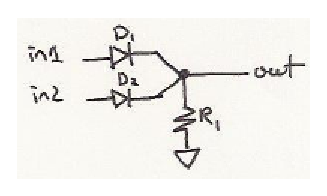
\includegraphics{images/DLor.eps}&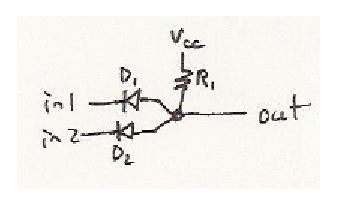
\includegraphics{images/DLand.eps}\\
\end{tabular}
\end{center}
\end{figure}
Consider the circuit in Figure~\ref{f:DL_or}.  If either $in_1$ or $in_2$ is high, the corresponding diodes ($D_1$ or $D_2$ respectively) turns on, making the output high.  Since the output will be about 0.6v less than the input you can't put too many of these in series before the logic level drops below useful levels.  If both inputs are off then both diodes don't conduct and the resistor to ground ($R_1$) pulls the output down to a low output (hence the name pull down resistor).  The circuit is thus an \textbf{or} gate.

Now consider the circuit in Figure~\ref{f:DL_and}.  If either $in_1$ or $in_2$ is low, the corresponding diodes ($D_1$ or $D_2$ respectively) turns on, making the output low, though it will be about 0.6v higher than the inputs so just like with the \textbf{or} gate, you can't do too many of these in series.  If by inputs are high, then both diodes are off and the output is isolated from the input.  The resistor to $V_{cc}$ pulls the output up (hence the name, pull up resistor).  The gate is thus an \textbf{and} gate.


\section{Resistor Transistor Logic}
Resistor Transistor Logic, (RTL) replaces the diodes of DL with transistors, which allowed for negation.  This is thus the first full logic family.


\section{Diode Transistor Logic}


\begin{figure}
\begin{center}
\caption{Diode Transistor Logic \textbf{Nand} Gate.}\label{f:DTL_nand}
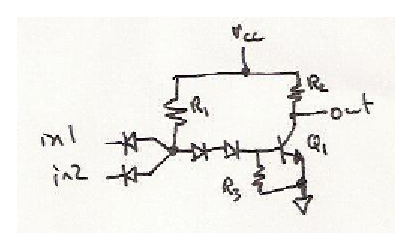
\includegraphics{images/DTLnand.eps}
\end{center}
\end{figure}

\section{Transistor Transistor Logic}
Transistor transistor logic (TTL) is arguably the most famous logic family.  It has been used for around 40 years, and can still be purchased today.  It is reasonably fast, has good noise rejection, and has good protection from static.  A large number of interfaces are TTL compatible, so even when the components are not used, its design implications are still felt.  The venerable 7400 and 5400 (milspec\footnote{Milspec means it is built to military specification, which would be enough to be noteworthy, but milspec parts are useful in hazardous environments, such as space, marine (water and saline), industrial fabrication environments, extreme temperature ranges, etc.}) series are the most famous TTL components, and they have been used widely in engineering labs since I was in school way back when...  If you want to see what components were in the series, see Appendix~\ref{c:7400}.



\begin{figure}
\begin{center}
\caption{Transistor Transistor Logic \textbf{Nand} Gate.}\label{f:TTL_nand}
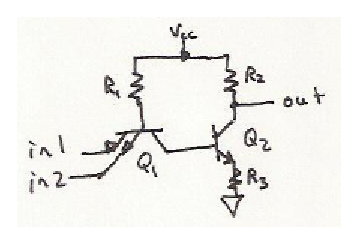
\includegraphics{images/TTLnand.eps}
\end{center}
\end{figure}

\subsection{Open Collector Outputs}
If you noticed in earlier logic families, typically the collector of the output transistor is connected to power by a pull-up transistor, and without it the ``high'' output would not function correctly (it would be a weak, floating high).  Since all the outputs use one, you could omit the resistor, and then wire the outputs together, and put an external pull-up.  Such an output is ``open collector'' and they allow you to do active-low wired-OR and active-high wired-AND functionality.  Wired gates are ``gates'' formed by wiring the outputs together, so you get a free gate.  If you were to try this with driven outputs, you would get a short as both high and low are typically driven.  Open collector outputs are generally slow, but proper resistor selection can improve things, and you can get two levels of logic for one level, which also saves time.  I would advise against them unless you really know what you are doing and why.  If you need to use them, the pull-up resistor is generally sized by calculating the minimum and maximum values per below.
\begin{eqnarray}
R_{max} &=& \frac{\min{(V_{cc})}-V_{OH}}{\sum{\max{(I_{OH})}}+\sum{\max{(I_{IH})}}}\\
R_{min} &=& \frac{\max{(V_{cc})}-V_{OL}}{I_{OL}-\sum{\max{(I_{IL})}}}
\end{eqnarray}
where, $V_{cc}$ is the supply voltage, $V_{OH}$ is the high output voltage of the gate, $I_{OH}$ is the high output current for every gate whose outputs are connected to the pull-up resistor, $I_{IH}$ is the high input current of every gate whose input is connected to the pull-up resistor, $I_{OL}$ is the low output current of the gate, and $I_{IL}$ is the low input current for every gate hooked to the pull-up resistor.  This might look fancy, but it is actually just Ohm's law ($R=V/I$ in this case), where the voltage is the difference from the output to the supply, and the current must consider all the possible currents.  We then maximize the top and minimize the bottom and vice versa to get our extreme cases.  Memorizing this would be tough, understanding it is easy and from this it can be easily recreated.


\begin{figure}
\begin{center}
\caption{Transistor Transistor Logic \textbf{Nand} Gate with Open Collector Output.}\label{f:TTL_nand_opencollector}
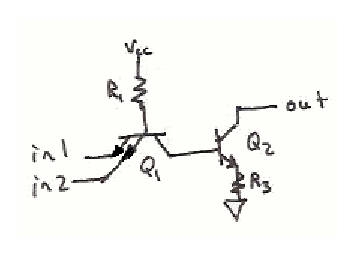
\includegraphics{images/TTLnand_opencollector.eps}
\end{center}
\end{figure}

\subsection{Totem Pole Outputs}
Instead of trying to take advantage of wired logic through a pull-up, we could consider how can we make the outputs switch as fast as possible.  To do this we would need to pull up and down with separate transistors, so that we could quickly drive the output high or low.  This is what totem pole outputs does.  It is called totem pole outputs because the output transistors are on top of each other like a totem pole.

\begin{figure}
\begin{center}
\caption{Transistor Transistor Logic \textbf{Nand} Gate with Totem Pole Output.}\label{f:TTL_nand_totem}
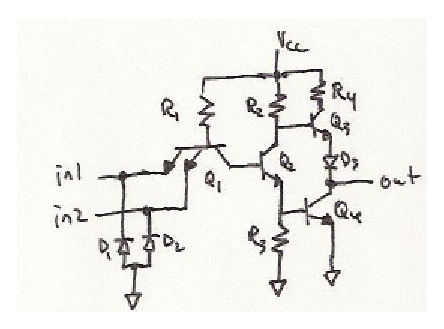
\includegraphics{images/TTLnand_totempole.eps}
\end{center}
\end{figure}

\subsection{Tristate Outputs}

\begin{figure}
\begin{center}
\caption{Transistor Transistor Logic \textbf{Nand} Gate with Tristate Output.}\label{f:TTL_nand_tristate}
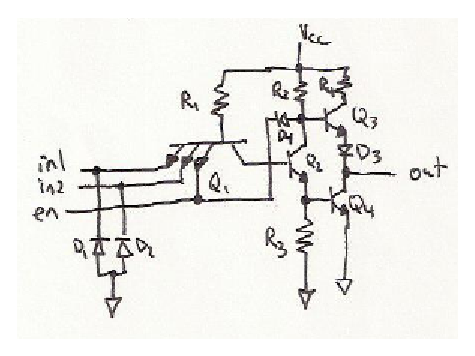
\includegraphics{images/TTLnand_tristate.eps}
\end{center}
\end{figure}




\section{CMOS Families}

\section{Static CMOS}

Static CMOS is the basic type, and aims at reliable, robust circuits.

\section{Dynamic CMOS}

Dynamic CMOS is designed to be small, fast, and low power.  Examples include PE Logic and Domino Logic, and require timing.  The key idea is to precharge and time the discharge to ensure that transitions occur quickly.  For instance Domino logic includes an inverter between gates to quickly change and cause a ripple of discharges from one stage to the next, thus falling like dominos\footnote{Yes dominos like the tile game, not the fast, cheap pizza. :)}.

\section{Interfacing}

There are a lot of logic families out there so I will only cover the most common ones in this section, the rest can be handled in similar ways, you just need to know the standard considerations of voltages (not just min and max but also the logic levels), current (input and output at high and low levels), impedance (not always needed but can be important on bus lines and such), floating outputs (high, low, or not at all), timing (rise time, fall time, latency, etc.), and data rates (really this is an implication of timing, but it is big enough to be mentioned separately).  It is helpful to know if the circuits you are interfacing are switching ground or power, as you can make a more reliable circuit using this information (i.e. you do the same in your circuit, which will be more compatible and thus also more reliable as it will not run into as many glitches caused by misreading a voltage level.).  The basic requirements to call two chips compatible are:

\begin{tabular}{rcl}
Driver Output  && Load Input \\
$V_{OH_{max}}$ & $<$ & $V_{IH_{max}}$\\
$V_{OH_{min}}$ & $>$ & $V_{IH_{min}}$\\
$V_{OL_{max}}$ & $<$ & $V_{IL_{max}}$\\
$V_{OL_{min}}$ & $>$ & $V_{I_{min}}$\\
$-I_{OH_{max}}$ & $>$ & $I_{IH_{max}}$\\
$I_{OL_{max}}$ & $>$ & $-I_{IL_{max}}$\\
\end{tabular}

The first two rows require that the high (true in positive logic) output voltage range must be contained in the high input voltage range, so that any $H$ produced is correctly received.  The next two lines do the same thing for the low values.  The last two are to ensure that the driving chip can supply the needed current for a $H$ and sink the needed current for a $L$.  Note the negative signs are present because they flow out of the corresponding terminals rather than in.  Level shifters can be placed between to meet voltage requirements, or current amplifiers/buffer stages can be used to meet current requirements.  Typically, the first requirement is met by keeping the supply voltage the same, provided they can both take the same supply voltage.  Similarly the fourth requirement is met by providing both the same ground.  The last two requirements need to be verified for the entire load they are driving (fan-out and fan-in problems).

Before you design a circuit to interface, you should check if there is a device that already does the interfacing.  In many cases there are devices designed for interfacing.  For instance, between the old TTL family and the newer CMOS families (C, HC, AC, ACH, etc.), there are T versions (CT, HCT, ACT, ACHT, etc.) that can drop in replace the old TTL components, or one of the T devices can sit between the families and convert (say a buffer or two inverters).  This is by far the easiest way to do the conversion, and I would do it this way unless forced to do otherwise.  It is useful to know how to convert, should you ever have to, so below are the basics.

If you are straight converting signals, you often want to go through two inverters\footnote{The inverters buffer the input.  Don't use an actual buffer because a buffer is slower than an inverter, so buffers should be avoided unless absolutely needed.  Basically, you put an inverter of the same logic type of the output immediately after the output and an inverter of the same logic type as the input immediately before the input.}, as these devices as they are often used for this purpose, they are frequently designed to handle input and output.  Note that you do not have to use inverters, they are a protection layer.  The inverters serve as sacrificial elements (one for each logic family) to protect the circuits they are interfacing.  Frequently you put them and any other interfacing hardware on a shim board, then if anything gets damaged it is the shim, not the original circuit.

Let's pick up the case mentioned above, where we wanted to go from an old TTL output to a newer CMOS input (say from a 74LS to a 74HC), but assume for some reason, we didn't just want to us a 74HCT to interface.  We would need three circuit elements: a but would also need a pull up resistor of about 1k between them for two reasons.  First, the voltage levels are incompatible, particularly at the high range, and the pull up solves this.  Second, the pull up resistor is used to guarantee the input does not stay in the dangerous 0.8v to 2.0v range\footnote{In the transition voltage range the P-channel to Vcc and the N-channel to ground can both be open, creating a path from Vcc to ground.  This causes a current spike which can damage circuits if it is around too long.  This happens every transition between high and low, but in the new CMOS families transitions are so fast the time of current spike is thus so short it does not effect things. The TTL output is slower and thus can allow significant damage.  A pull up (or pull down if you want the default low) resistor solves this problem.}.  To calculate the pull-up resistor more precisely you can use
\begin{eqnarray}
R_{pull-up} &\geq& \frac{V_{cc}max-V_{TTL\; Low\; Output}}{I_{TTL\; Low\; Output} + (num\; inputs)I_{CMOS\; Low\; Input}}\label{eq-resistor-pull-up-min}\\
R_{pull-up} &\leq& \frac{V_{cc}-V_{CMOS\; Input\; High}}{(num\; inputs)I_{CMOS\; Input\; High}}\label{eq-resistor-pull-up-max}
\end{eqnarray}
Usually the minimum value is in the mid to high hundreds so a 1k resistor is a good guess up till about $num\; inputs=8$, past that I would guess 2k till about $num\; inputs=16$, I would not drive more than 16 gates directly with anything at the moment (theoretically you can but current, heat, and transients become big problems).  The input current of CMOS devices is very small, so it can usually be ignored in the lower bound, and will cause the upper bound to be large (but finite).  As the number of devices grows it cannot be ignored and at around $num\; inputs=18$ there is a crossover, thus no pull-up resistor will work.  You should calculate the minimum and maximum for any problem to ensure there is a feasible region and you are in it.

Depending on the circuit, you might also have to guarantee a particular rise time (the second reason we wanted a pull-up).  In this case we have a simple first order\footnote{This is the solution of a first order derivative equation for the rise time of a driven RC circuit.  Theoretically they covered a lot of this in your physics sequence.} equation
\begin{eqnarray}
V_{CMOS\; Input\; High} &=& V_{CC}\left(1-e^{-\frac{t}{C\cdot R_{pull-up}}}\right)
\end{eqnarray}
where $t$ is the desired rise time, and $C$ is the total capacitance of the circuit, which is the sum of the output capacitance of the driving circuit, the input capacitance of the receiving circuits, and the capacitance of the line (often negligible but not always, it is probably about 1pF/cm).  You can solve this for the value of $R_{pull-up}$.  All of this assumed open-collector output (nothing driving high).  If something is driving the circuit high, the pull-up resistor only has to account for the missing voltage.  For instance totem pole output (typical for many TTL such as the LS family logic gates) is driven to at least 2.7 volts in around 10ns.  Given some driven output voltage the equation for the pull-up resistor is
\begin{eqnarray}
V_{CMOS\; Input\; High}-V_{Driven\; Output} &=& (V_{CC}-V_{Driven\; Output})\left(1-e^{-\frac{t}{C\cdot R_{pull-up}}}\right).
\end{eqnarray}
Again solve for $R_{pull-up}$ and then ensure it falls between the minimum (Eq.~\ref{eq-resistor-pull-up-min}) and maximum (Eq.~\ref{eq-resistor-pull-up-max}).

If we were going the other way, we could just directly connect them, as long as we were in the fan-out restrictions, which is at least 10 gates for LS-TTL or 2-4 gates for TTL.  Often designers put an additional CMOS buffer, say a 4096, for timing input to the slower TTL circuits.  Note the data rates must be compatible, or no buffer will be able to solve incompatible data rates for continuous data streams.

As an interesting side note TTL at 5v is directly compatible, both ways with CMOS at 3v.  Fan in and out restrictions still apply.

It is worth noting that CMOS has a wide range of voltage operation, so it is not uncommon to have to convert voltage ranges.  Resistor voltage dividers are common for going down, and amplifier circuits, such as an open drain CMOS device with a pull-up resistor.  As a particularly interesting case is ECL, which is usually run between 0v and -5.2v so the voltage differences and potential logic inversions need to be handled, or you can just run the CMOS from the same supply, and then just use diodes on the interface for protection. 